\chapter{\textbf{Resultados}} % Este comando é utilizado para criar capítulos
\sloppy % Corrige estouro de linhas

\section{Aplicativo}

Todo o processo de construção do aplicativo foi baseado na metodologia utilizada na disciplina de Laboratório de Engenharia de Software \cite{rupLes}. Para tanto, foram realizadas as seguintes etapas:

\subsection{Levantar Requisitos (Visão Geral)}

Nesta etapa foi realizado um levantamento de funcionalidades básicas necessárias junto a empresa responsável pelo gerenciamento dos dados dos alunos. A partir desta, foi elaborado uma descrição geral sobre o escopo do aplicativo.

\subsection{Elaborar Modelo Conceitual}

A construção do modelo conceitual foi baseada no levantamento realizado na etapa anterior, levando em consideração as informações disponibilizadas pela base de dados cedida, conforme a figura \ref{figura:modelo_conceitual}.

\begin{figure}[H]
	\caption{Modelo Conceitual.}
	\centering % para centralizarmos a figura
	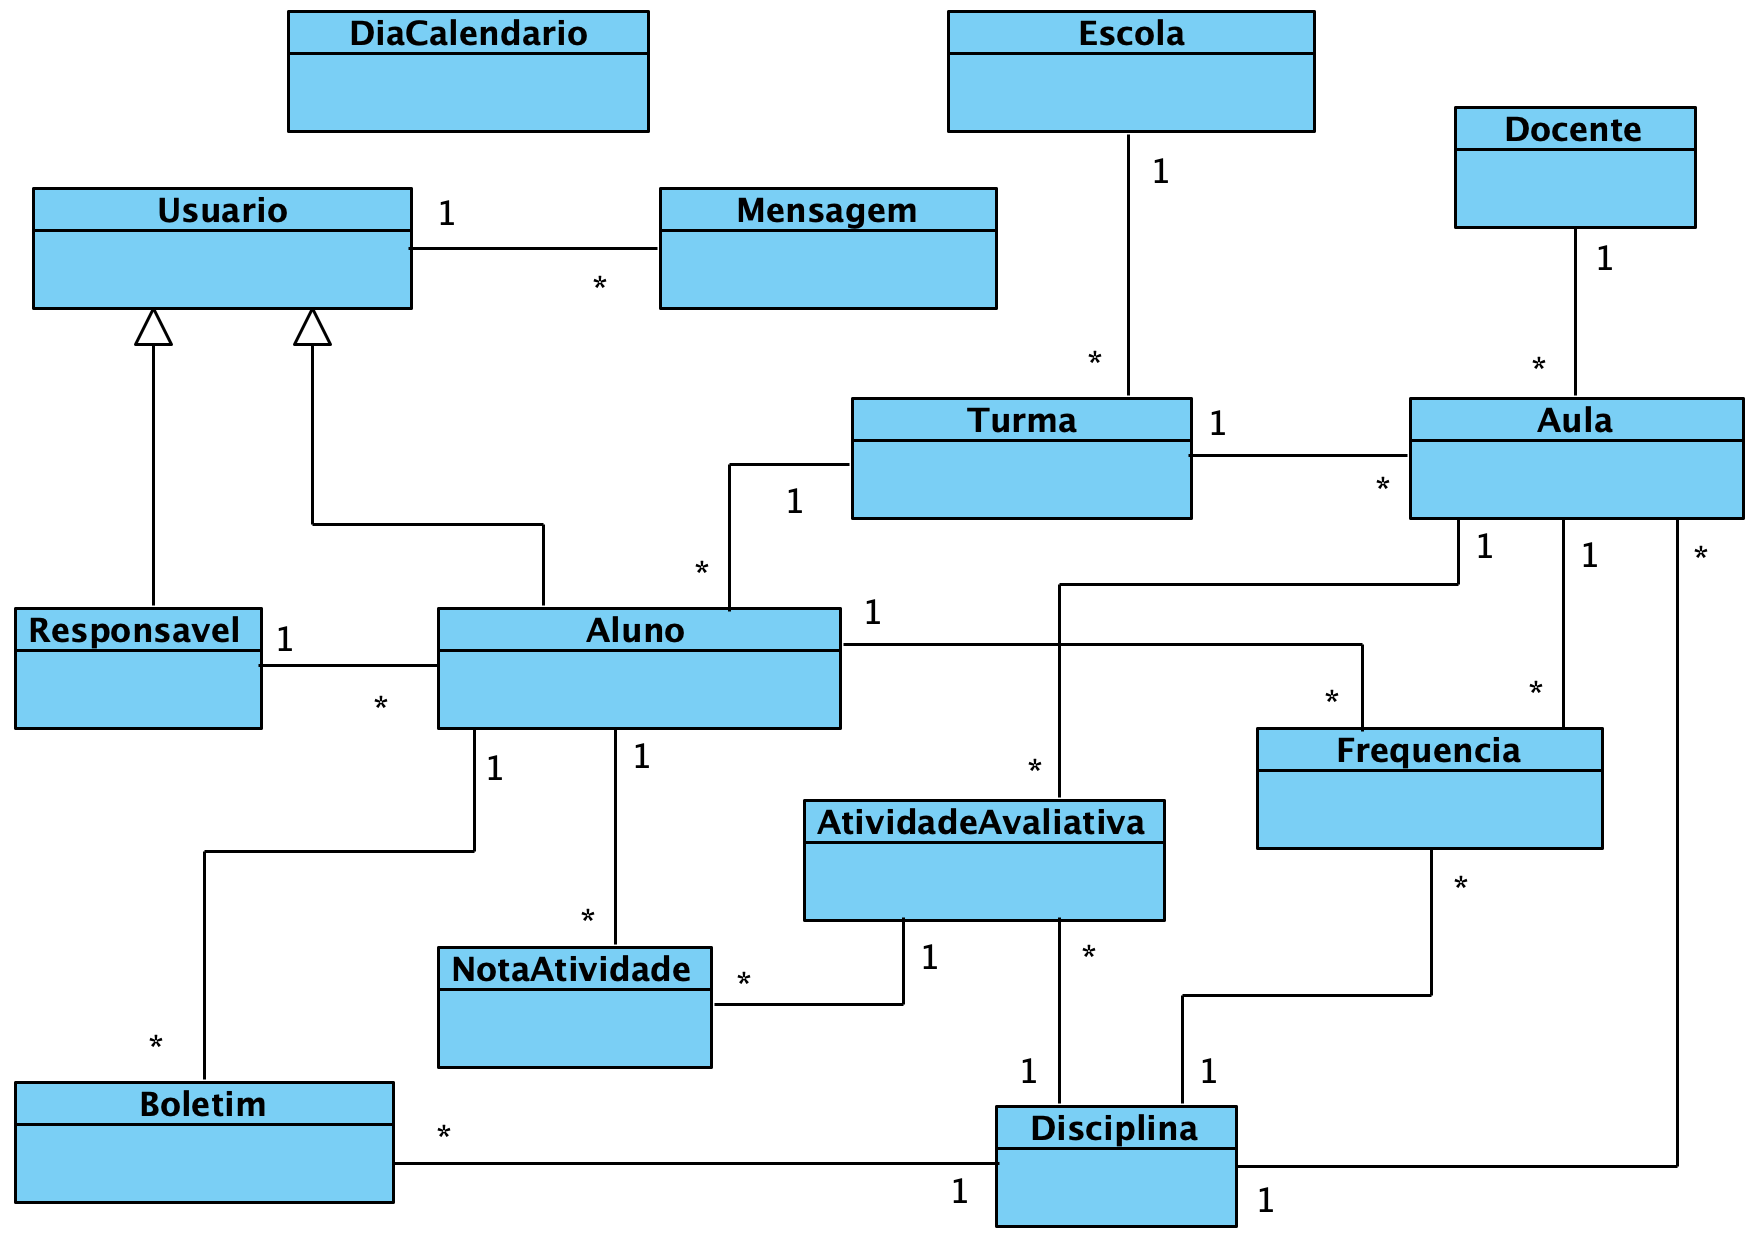
\includegraphics[width=13.7cm]{resources/modelo_conceitual.png} % leia abaixo
	\label{figura:modelo_conceitual}
	\captionsetup{singlelinecheck = false, format= hang, justification=raggedright, labelsep=space, width=13.7cm}
	\caption*{\footnotesize Fonte: O Autor.}
\end{figure}

\subsection{Levantar Requisitos}

Nesta etapa foi produzido o documento de requisitos. Ao todo, foram identificados 12 requisitos, sendo 2 de processos de negócio e 10 de listagens. Todos os requisitos foram definidos a partir de reuniões realizadas com a empresa responsável por ceder os dados.

\subsection{Organizar Requisitos}

Nesta etapa, os requisitos forma organizados entre as categorias: processos de negócios e listagens/relatórios.

Os requisitos de processos de negócio foram, respectivamente: entrar no sistema e sair do sistema.

Os requisitos de listagem foram, respectivamente: listar alunos por responsável, listar grade horária por aluno, listar atividades avaliativas por aluno e trimestre, listar frequências por aluno, disciplina e trimestre, listar boletim por aluno e trimestre, listar dados do aluno, listar dados da emeb por aluno, listar mensagens por aluno, listar mensagens por responsável, listar calendário acadêmico.

\subsection{Elaborar diagrama de classes de projeto}

Nesta etapa foi elaborado o diagrama de classes de projeto, considerando os dados a serem utilizados no aplicativo, levantados no documento de requisitos.

\begin{figure}[H]
	\caption{Diagrama de Classe.}
	\centering % para centralizarmos a figura
	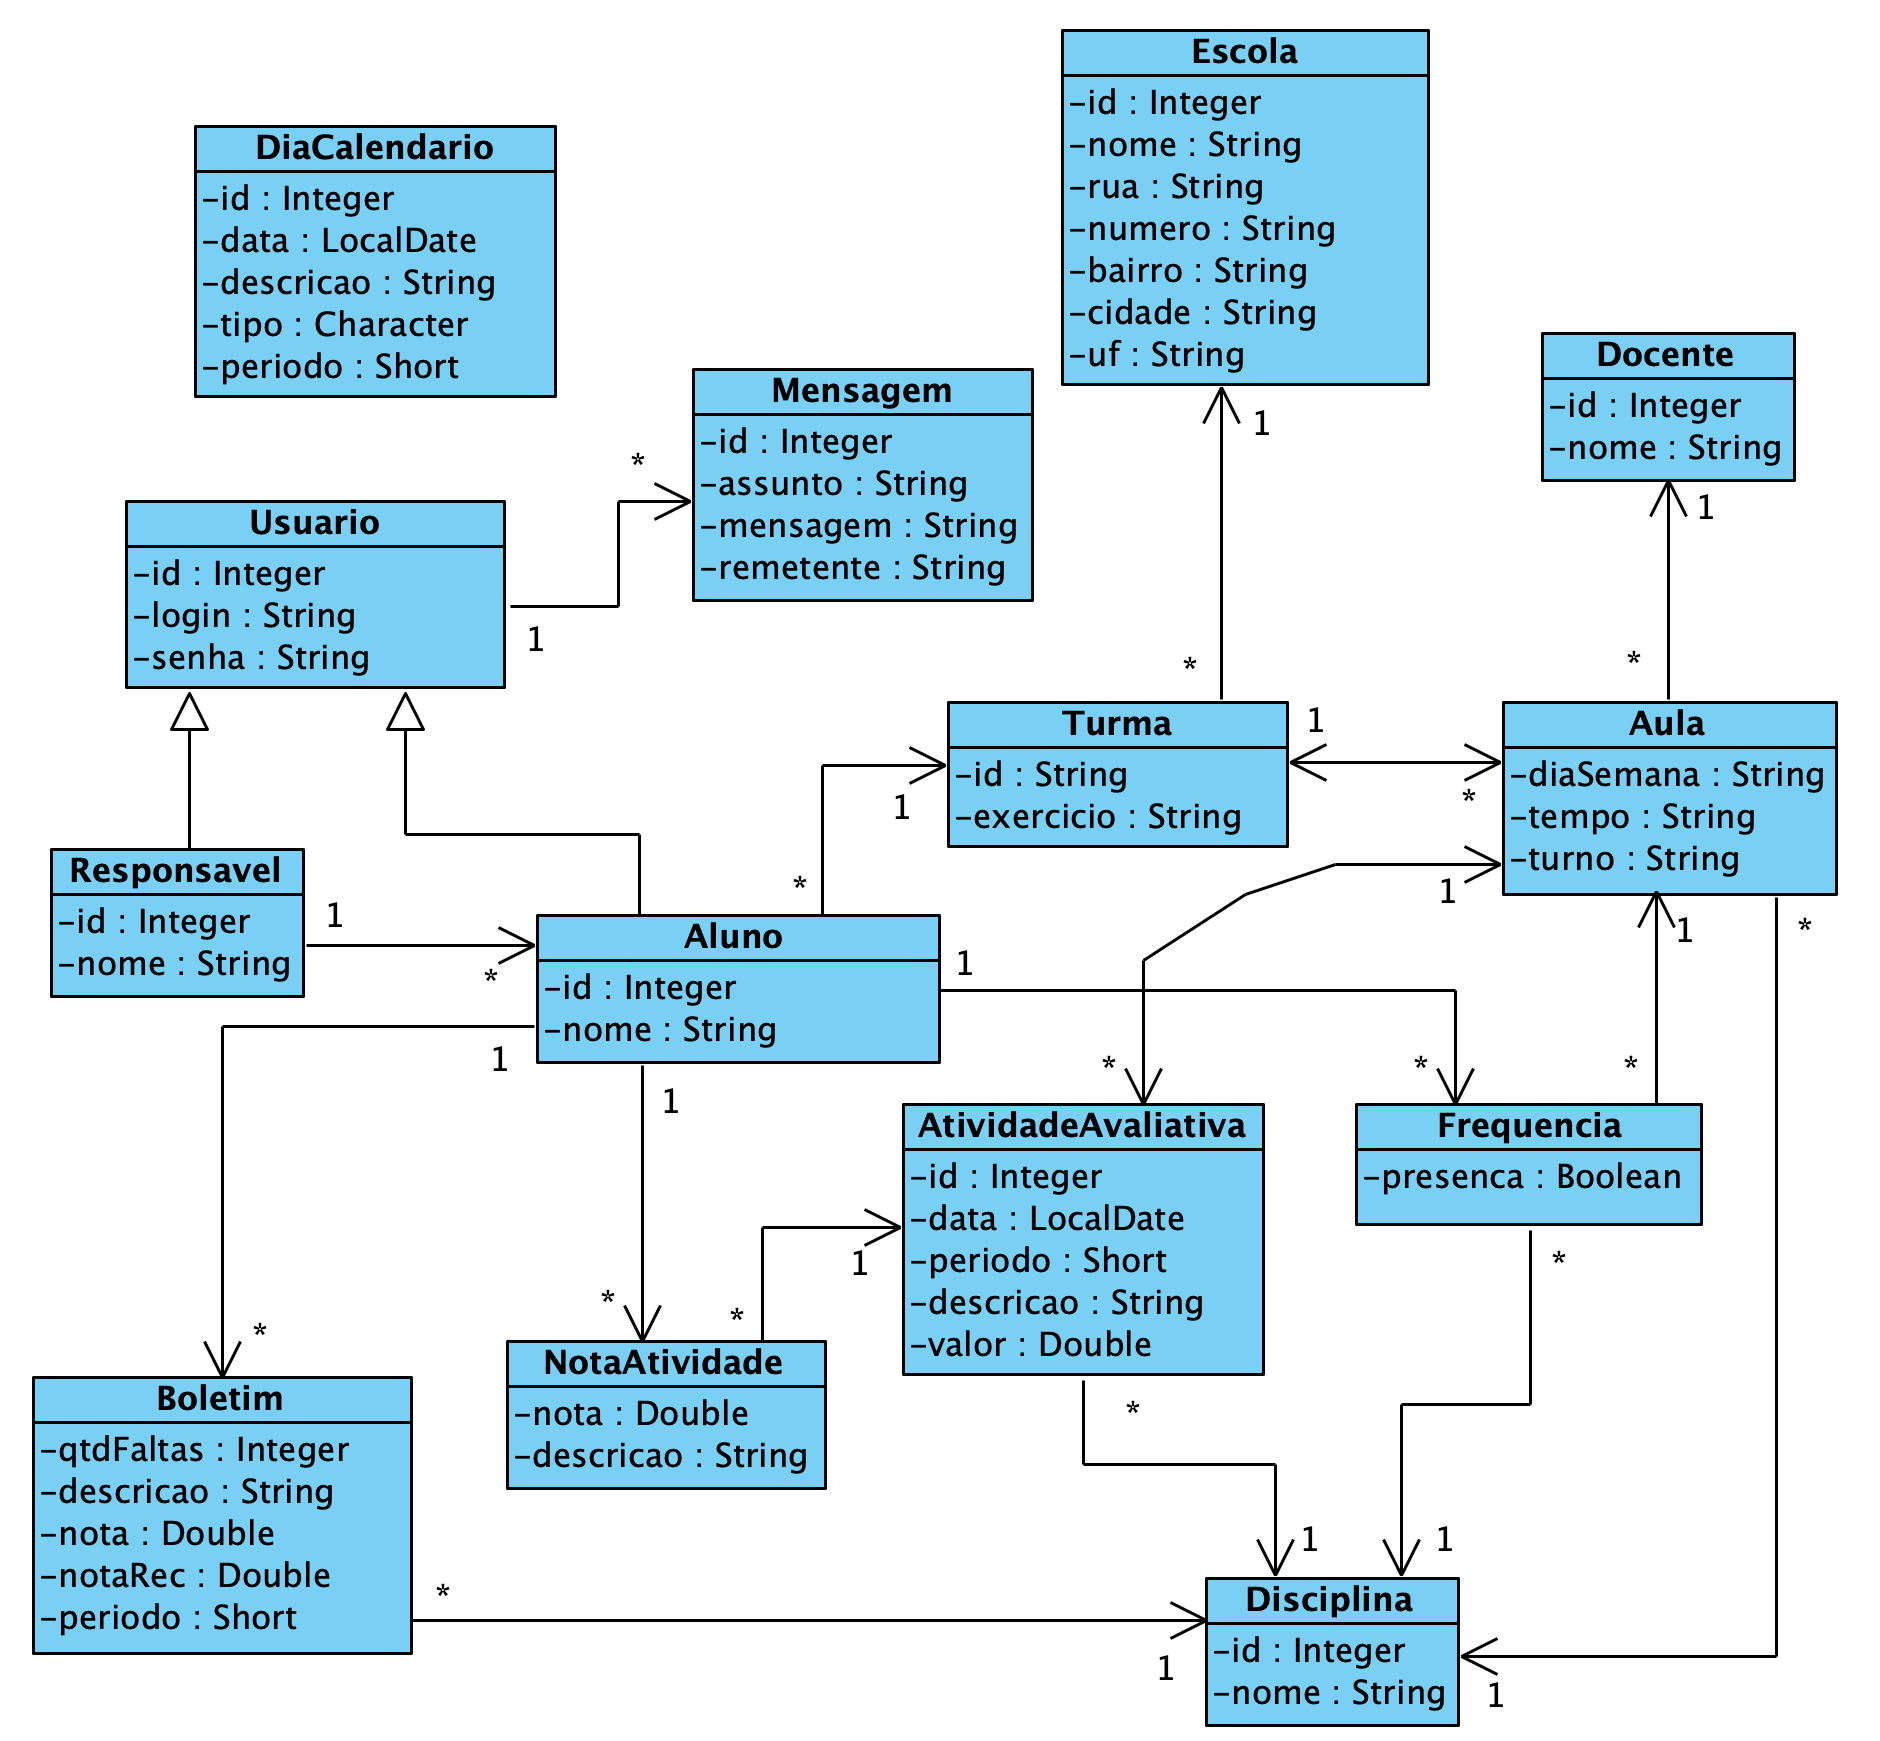
\includegraphics[width=16cm]{resources/classes_projeto.png} % leia abaixo
	\label{figura:diagrama_classe}
	\captionsetup{singlelinecheck = false, format= hang, justification=raggedright, labelsep=space, width=16cm}
	\caption*{\footnotesize Fonte: O Autor.}
\end{figure}

\subsection{Implementar}

\subsubsection{Aplicativo Mobile}

O aplicativo mobile foi implementado utilizando a linguagem Typescript, através do \textit{framework} de desenvolvimento Ionic, na versão 4. Foi utilizado o editor de texto o Visual Studio Code para a codificação desta etapa. A tabela \ref{tabela:app_organizacao} demonstra a organização básica dos principais diretórios do projeto, bem como suas respectivas descrições: 

\renewcommand{\arraystretch}{1.5}
\begin{table}[H]
    \small
	\centering
	\caption{Organização de Diretórios do Aplicativo Mobile.}
	\label{tabela:app_organizacao}
	\begin{tabular}{c l}
	    \hline
		\multicolumn{1}{l|}{\textbf{Diretório}} & \multicolumn{1}{c}{\textbf{Descrição}}\\
		\hline
		models & Classes de mapeamento de dados retornados pela API  \\
		pages & Telas do aplicativo \\
		services & Classes de acesso ao Web Service \\
		\hline
	\end{tabular}
	\captionsetup{singlelinecheck = false, format= hang, justification=raggedright, labelsep=space, width=11.9cm}
	\caption*{\footnotesize Fonte: O Autor.}
\end{table}
\renewcommand{\arraystretch}{1}

A seguir serão apresentadas as telas implementadas para as funcionalidades definidas no escopo do projeto:

\begin{itemize}
	\item Login (figura \ref{figura:login}): tela de login do aplicativo;
	\item Menu Principal (figura \ref{figura:menu_principal}): contém opções de acesso para funções gerais do sistema e dados básicos do perfil do usuário logado;
\end{itemize}

\begin{figure}[H]
    \begin{minipage}[b]{0.45\linewidth}
        \caption{Tela de Login.}
    	\centering % para centralizarmos a figura
    	\shadowbox{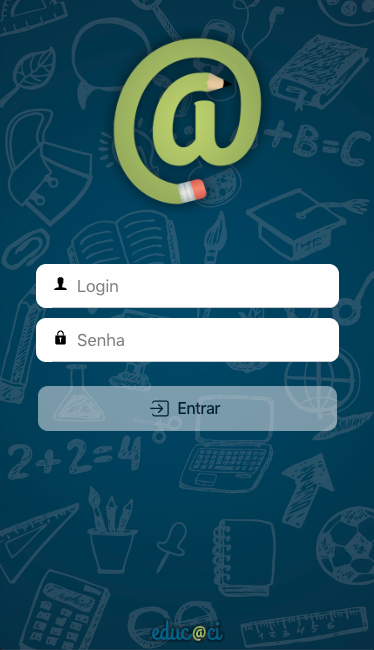
\includegraphics[width=6cm]{resources/prints_app/login.png}} % leia abaixo
    	\label{figura:login}
    	\captionsetup{singlelinecheck = false, format= hang, justification=raggedright, labelsep=space, width=6.5cm}
    	\caption*{\footnotesize Fonte: O Autor.}
    \end{minipage}
    \hspace{0.5cm}
    \begin{minipage}[b]{0.45\linewidth}
        \caption{Menu principal.}
    	\centering % para centralizarmos a figura
    	\shadowbox{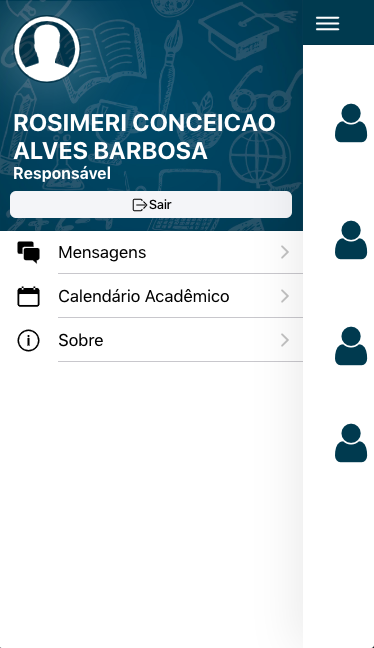
\includegraphics[width=6cm]{resources/prints_app/menu_principal.png}} % leia abaixo
    	\label{figura:menu_principal}
    	\captionsetup{singlelinecheck = false, format= hang, justification=raggedright, labelsep=space, width=6.5cm}
    	\caption*{\footnotesize Fonte: O Autor.}
    \end{minipage}
\end{figure}

\begin{itemize}
	\item Listagem de alunos (figura \ref{figura:lista_alunos}): disponível apenas para usuários com perfil de responsável, esta funcionalidade lista todos os alunos vinculados ao perfil logado, permitindo o acesso aos dados de todos os alunos listados;
	\item Perfil do aluno (figura \ref{figura:perfil_aluno}): contém informações gerais sobre um aluno, bem como as opções de acesso aos dados acadêmicos do mesmo;
\end{itemize}

\begin{figure}[H]
    \begin{minipage}[b]{0.45\linewidth}
        \caption{Listagem de alunos.}
    	\centering % para centralizarmos a figura
    	\shadowbox{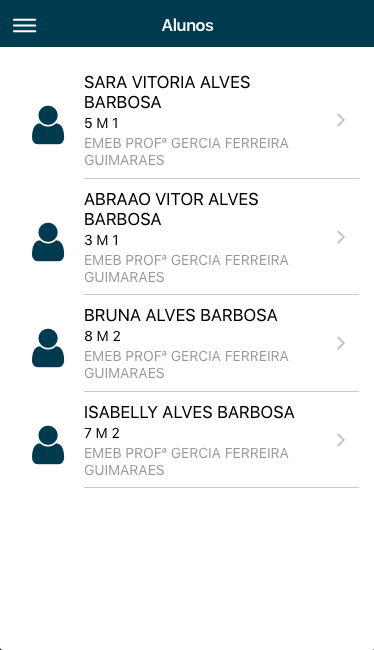
\includegraphics[width=6cm]{resources/prints_app/listagem_alunos.png}} % leia abaixo
    	\label{figura:lista_alunos}
    	\captionsetup{singlelinecheck = false, format= hang, justification=raggedright, labelsep=space, width=6.5cm}
    	\caption*{\footnotesize Fonte: O Autor.}
    \end{minipage}
    \hspace{0.5cm}
    \begin{minipage}[b]{0.45\linewidth}
        \caption{Perfil de um aluno.}
    	\centering % para centralizarmos a figura
    	\shadowbox{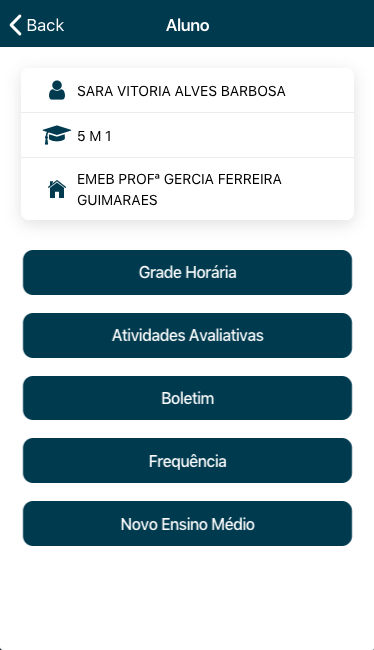
\includegraphics[width=6cm]{resources/prints_app/perfil_aluno.png}} % leia abaixo
    	\label{figura:perfil_aluno}
    	\captionsetup{singlelinecheck = false, format= hang, justification=raggedright, labelsep=space, width=6.5cm}
    	\caption*{\footnotesize Fonte: O Autor.}
    \end{minipage}
\end{figure}

\begin{itemize}
	\item Listagem de dias da grade horária (figura \ref{figura:grade_dias}): quando o usuário seleciona a função grade horária, a partir do perfil de um aluno (figura \ref{figura:perfil_aluno}), são listados todos os dias disponíveis em que há horários registrados com aulas para o aluno;
	\item Grade horária por dia (figura \ref{figura:grade}): ao selecionar um dia específico na tela representada na figura \ref{figura:grade_dias}, são mostrados os horários registrados com aulas para o aluno por tempo, indicando a disciplina e o docente respectivos;
\end{itemize}

\begin{figure}[H]
    \begin{minipage}[b]{0.45\linewidth}
        \caption{Listagem de dias da grade horária.}
    	\centering % para centralizarmos a figura
    	\shadowbox{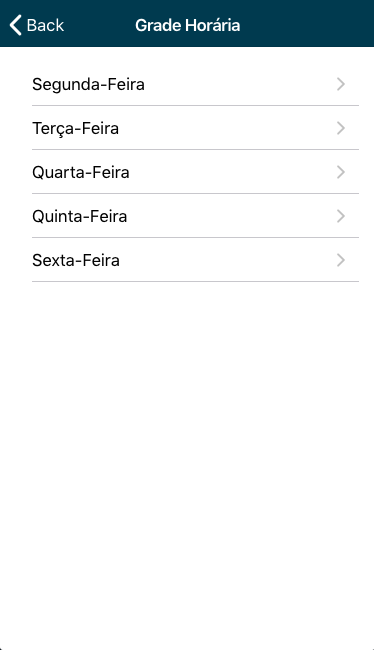
\includegraphics[width=6cm]{resources/prints_app/grade_horaria1.png}} % leia abaixo
    	\label{figura:grade_dias}
    	\captionsetup{singlelinecheck = false, format= hang, justification=raggedright, labelsep=space, width=6.5cm}
    	\caption*{\footnotesize Fonte: O Autor.}
    \end{minipage}
    \hspace{0.5cm}
    \begin{minipage}[b]{0.45\linewidth}
        \caption{Exibição do horário de aulas por dia da grade horária.}
    	\centering % para centralizarmos a figura
    	\shadowbox{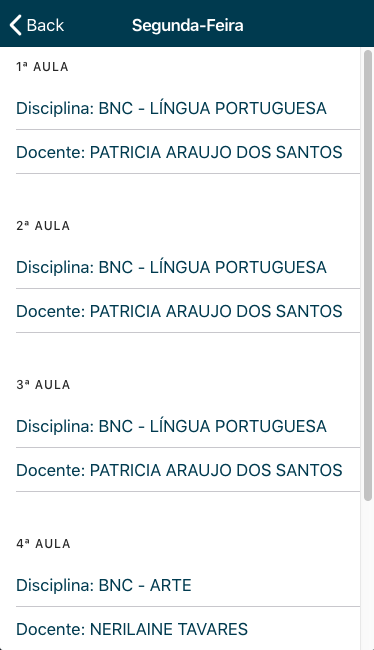
\includegraphics[width=6cm]{resources/prints_app/grade_horaria2.png}} % leia abaixo
    	\label{figura:grade}
    	\captionsetup{singlelinecheck = false, format= hang, justification=raggedright, labelsep=space, width=6.5cm}
    	\caption*{\footnotesize Fonte: O Autor.}
    \end{minipage}
\end{figure}

\begin{itemize}
	\item Listagem de atividades avaliativas (figura \ref{figura:ativ_aval}): lista atividades avaliativas programadas por trimestre, bem como seus dados respectivos;
	\item Boletim Trimestral (figura \ref{figura:boletim}): exibe o boletim de um aluno dado um trimestre selecionado, com suas devidas disciplinas, notas e faltas;
\end{itemize}

\begin{figure}[H]
    \begin{minipage}[b]{0.45\linewidth}
        \caption{Listagem de atividades avaliativas.}
    	\centering % para centralizarmos a figura
    	\shadowbox{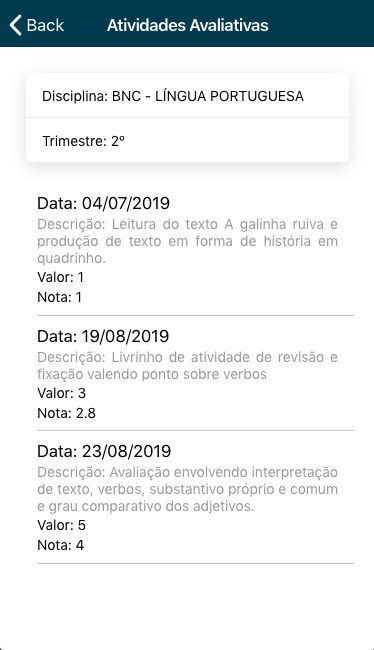
\includegraphics[width=6cm]{resources/prints_app/atividades_avaliativas.png}} % leia abaixo
    	\label{figura:ativ_aval}
    	\captionsetup{singlelinecheck = false, format= hang, justification=raggedright, labelsep=space, width=6.5cm}
    	\caption*{\footnotesize Fonte: O Autor.}
    \end{minipage}
    \hspace{0.5cm}
    \begin{minipage}[b]{0.45\linewidth}
        \caption{Boletim trimestral.}
    	\centering % para centralizarmos a figura
    	\shadowbox{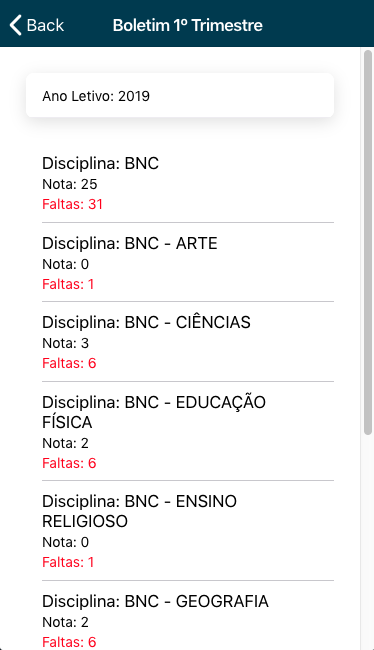
\includegraphics[width=6cm]{resources/prints_app/boletim.png}} % leia abaixo
    	\label{figura:boletim}
    	\captionsetup{singlelinecheck = false, format= hang, justification=raggedright, labelsep=space, width=6.5cm}
    	\caption*{\footnotesize Fonte: O Autor.}
    \end{minipage}
\end{figure}

\begin{itemize}
	\item Listagem de frequências (figura \ref{figura:freq}): lista frequências do aluno por trimestre selecionado, indicando o conteúdo ministrado no dia e a quantidade de faltas;
	\item Calendário acadêmico (figura \ref{figura:calendario}): exibe todas as datas definidas para um ano letivo;
\end{itemize}

\begin{figure}[H]
    \begin{minipage}[b]{0.45\linewidth}
        \caption{Listagem de frequências.}
    	\centering % para centralizarmos a figura
    	\shadowbox{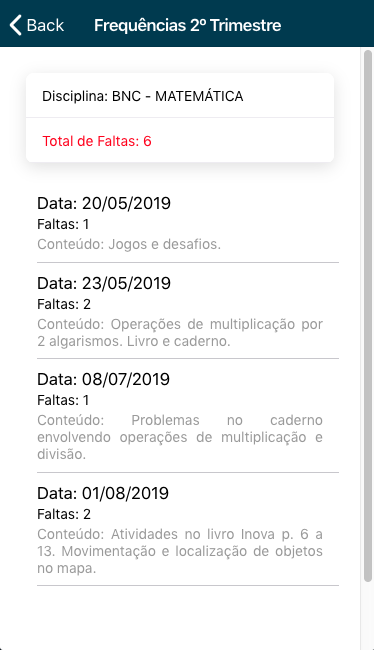
\includegraphics[width=6cm]{resources/prints_app/frequencias.png}} % leia abaixo
    	\label{figura:freq}
    	\captionsetup{singlelinecheck = false, format= hang, justification=raggedright, labelsep=space, width=6.5cm}
    	\caption*{\footnotesize Fonte: O Autor.}
    \end{minipage}
    \hspace{0.5cm}
    \begin{minipage}[b]{0.45\linewidth}
        \caption{Calendário acadêmico.}
    	\centering % para centralizarmos a figura
    	\shadowbox{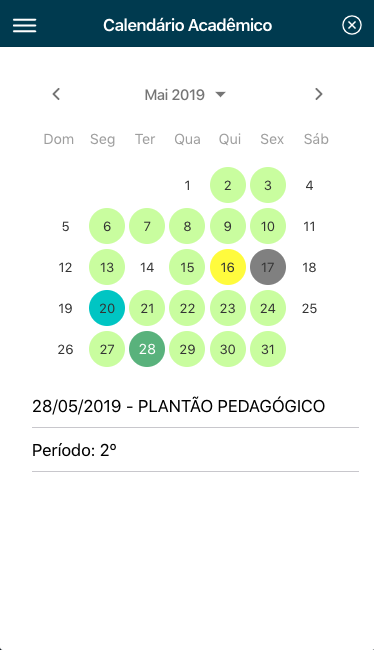
\includegraphics[width=6cm]{resources/prints_app/calendario_academico.png}} % leia abaixo
    	\label{figura:calendario}
    	\captionsetup{singlelinecheck = false, format= hang, justification=raggedright, labelsep=space, width=6.5cm}
    	\caption*{\footnotesize Fonte: O Autor.}
    \end{minipage}
\end{figure}

\begin{figure}[H]
	\caption{Mensagem.}
	\centering % para centralizarmos a figura
	\shadowbox{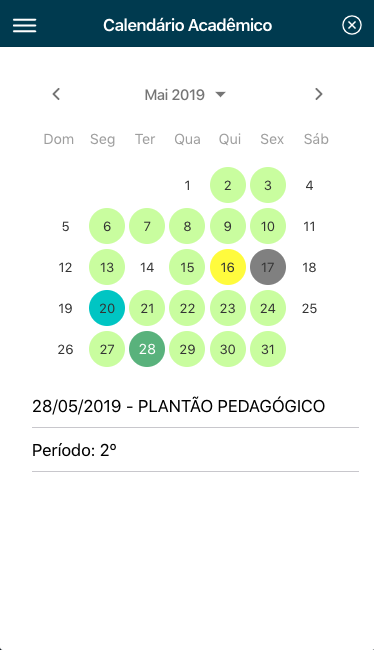
\includegraphics[width=6cm]{resources/prints_app/calendario_academico.png}} % leia abaixo
	\label{figura:treinamento}
	\captionsetup{singlelinecheck = false, format= hang, justification=raggedright, labelsep=space, width=6.5cm}
	\caption*{\footnotesize Fonte: O Autor.}
\end{figure}

\subsubsection{Web Service Restful}

A implementação do web service foi realizada utilizando a linguagem Java 1.8, e o framework Spring Boot na versão 2.1.0. Foi utilizado o IDE Netbeans 11.1 como ferramenta para codificação desta etapa. A organização do código da aplicação se dispõe em pacotes, tal como mostra a tabela \ref{tabela:webservice_package}.

\begin{table}[H]
    \small
	\centering
	\caption{Organização de pacotes do Web Service.}
	\renewcommand{\arraystretch}{1.5}
	\begin{tabular}{>{\centering}m{1.5in} >{\centering\arraybackslash}m{2.0in}}
	    \hline
		\multicolumn{1}{c|}{\textbf{Pacote}} 
		& \multicolumn{1}{c}{\textbf{Descrição}}\\
		\hline
		model & Classes de modelo  \\
		service & Classes de serviço, para eventuais regras de negócio \\
		resource & Classes controladoras, que recebem e respondem chamadas ao web service \\
		repository & Classes de acesso ao banco \\
		\hline
	\end{tabular}
	\label{tabela:webservice_package}
	\captionsetup{singlelinecheck = false, format= hang, justification=raggedright, labelsep=space, width=9.8cm}
	\caption*{\footnotesize Fonte: O Autor.}
\end{table}

A tabela \ref{tabela:webservice_servicos} apresenta o mapeamento de todos os serviços disponibilizados, especificando as URI de acesso, bem como seus respectivos métodos, tipos de retorno e descrições:

\begin{table}[H]
    \small
	\centering
	\caption{Mapeamento dos serviços do Web Service.}
	\renewcommand{\arraystretch}{1.5}
	\begin{tabular}{>{\centering}m{1.8in} >{\centering}m{0.5in} >{\centering}m{1.4in} >{\centering\arraybackslash}m{1.9in}}
	    \hline
		\multicolumn{1}{c|}{\textbf{URI}} 
		& \multicolumn{1}{c|}{\textbf{Método}}
		& \multicolumn{1}{c|}{\textbf{Retorno}}
		& \multicolumn{1}{c}{\textbf{Descrição}}\\
		\hline
		/login & POST & - & Realiza login através das credenciais do usuário \\
		/aluno/alun/\{id\}/\{ano\} & GET & List<Aluno> & Busca dados de um aluno por id e ano letivo \\
		/resp/\{id\}/\{ano\} & GET & List<Aluno> & Busca dados de alunos por id do responsável e ano letivo \\
		/aluno/grade/\{id\} & GET & List<Aula> & Busca aulas de uma grade horária por id do aluno \\
		/ativ/\{id\}/\{per\}/\{disc\} & GET & List<Atividade> & Busca atividades avaliativas por id do aluno, período e id da disciplina \\
		/ativ/\{id\}/\{per\} & GET & List<Disciplina> & Busca disciplinas para consulta de atividades avaliativas por id do aluno e período \\
		/aluno/boletim/\{id\}/\{per\} & GET & List<Boletim> & Busca boletins por id do aluno e período \\
		/freq/\{id\}/\{per\}/\{disc\}/total & GET & List<Frequencia> & Busca frequências por id do aluno, periodo e id da disciplina \\
		/freq/\{id\}/\{per\}/\{disc\}/total & GET & Integer & Busca total de frequências por id do aluno, periodo e id da disciplina \\
		/freq/\{id\}/\{per\} & GET & List<Disciplina> & Busca disciplinas para consulta de frequências por id do aluno e período \\
		/freq/\{id\}/\{per\}/total & GET & Integer & Busca total de faltas por id do aluno e período \\
		/cale/\{ano\} & GET & List<DiaCalendario> & Busca dias do calendário acadêmico por ano letivo \\
		/usuario/msg/\{id\} & GET & List<Mensagem> & Busca mensagens pelo id do usuário \\
		/aluno/classify/\{id\} & GET & double[] & Busca recomendação de área de aptidão com base no Novo Ensino Médio \\
		/resp/count & POST & - & Envia quantidade de cliques realizada pelo usuário com perfil de responsável \\
		\hline
	\end{tabular}
	\label{tabela:webservice_servicos}
	\captionsetup{singlelinecheck = false, format= hang, justification=raggedright, font=footnotesize, labelsep=space}
	\caption*{\footnotesize Fonte: O Autor.}
\end{table}

\subsection{Testar}

\subsection{Implantar}

\section{Módulo de Recomendação baseado em Redes Neurais}

A Implementação do módulo baseado em redes neurais foi implementada utilizando a biblioteca Weka, na versão 3.8.3. Para tal, foram executados os seguintes passos no processo de construção:

\subsection{Selecionar variáveis para o treinamento da rede}

Para a seleção de variáveis a serem utilizadas no treinamento foi realizado, sob auxílio de um pedagogo, dentre quarenta variáveis disponíveis na base de dados cedida, a seleção de dezenove parâmetros para  \ref{tabela:variaveis}.

\begin{table}[H]
    \small
	\centering
	\caption{Variáveis utilizadas no treinamento da rede.}
	\renewcommand{\arraystretch}{1.5}
	\begin{tabular}{>{\centering}m{1.8in} >{\centering\arraybackslash}m{4.2in}}
	    \hline
		\multicolumn{1}{c|}{\textbf{Variável}} 
		& \multicolumn{1}{c}{\textbf{Descrição}}\\
		\hline
		grau\textunderscore pai & Grau de escolaridade do pai \\
		grau\textunderscore mae & Grau de escolaridade da mãe \\
		duracao\textunderscore gestacao & Duração da gestação do aluno \\
		autismo & Indica se o aluno é portador de autismo \\
		superdotacao & Indica se o aluno possui superdotação \\
		bolsa\textunderscore familia & Indica se o aluno é participante programa Bolsa Família \\
		escola & Indica a escola onde o aluno estuda \\
		escola\textunderscore internet & Indica se a escola possui internet \\
		escola\textunderscore integral & Indica se a escola possui turno integral \\
		pai\textunderscore vivo & Indica se o pai é vivo \\
		mae\textunderscore viva & Indica se a mão é viva \\
		sexo & Indica o sexo do aluno \\
		percentual\textunderscore frequência & Indica o percentual de frequência do aluno considerando toda a sua vida acadêmica como estudante na rede de ensino \\
		media\textunderscore português & média das notas do aluno na disciplina de português (considerando todos os anos registrados) \\
		media\textunderscore matematica & média das notas do aluno na disciplina de matemática (considerando todos os anos registrados) \\
		media\textunderscore historia & média das notas do aluno na disciplina de história (considerando todos os anos registrados) \\
		media\textunderscore geografia & média das notas do aluno na disciplina de geografia (considerando todos os anos registrados) \\
		media\textunderscore ciências & média das notas do aluno na disciplina de ciências (considerando todos os anos registrados) \\
		cliques\textunderscore responsavel & quantidade de cliques ou interações realizadas pelo responsável do aluno junto ao aplicativo \\
		\hline
	\end{tabular}
	\label{tabela:variaveis}
	\captionsetup{singlelinecheck = false, format= hang, justification=raggedright, font=footnotesize, labelsep=space}
	\caption*{\footnotesize Fonte: O Autor.}
\end{table}

\subsection{Preparar o arquivo de treinamento}

O arquivo de treinamento foi elaborado a partir das variáveis selecionadas na etapa anterior. Os dados de inseridos no mesmo foram simulados, porém atendendo aos requisitos das variáveis.

\subsection{Realizar o treinamento da rede}

O processo de treinamento da rede foi realizado utilizando a ferramenta Weka Explorer, que realiza a leitura do arquivo de treinamento, exibindo as informações do mesmo de forma gráfica. Como algoritmo de treinamento foi utilizado o \textit{Multilayer Perceptron}. No decorrer do treinamento foram utilizadas várias configurações objetivando aumentar a taxa de acerto de classificação da rede. Na configuração final do treinamento, representada na figura \ref{figura:treinamento}, foram definidas três camadas escondidas de neurônios, sendo a quantidade deles em cada camada, respectivamente, 4, 29 e 19.

\begin{figure}[H]
	\caption{Configuração final do treinamento.}
	\centering % para centralizarmos a figura
	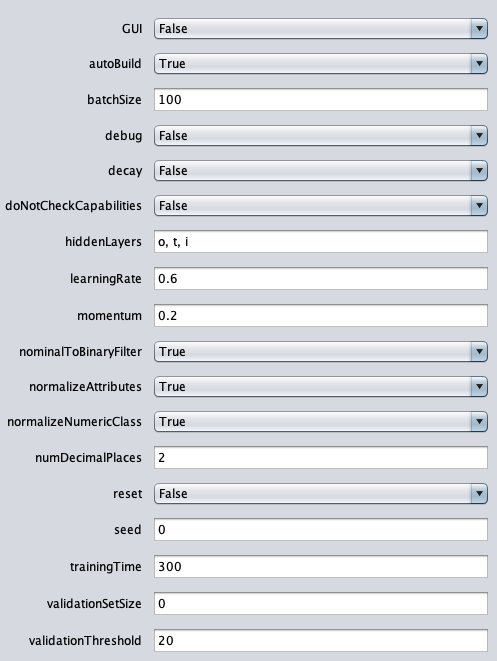
\includegraphics[width=11cm]{resources/treinamento_weka.png} % leia abaixo
	\label{figura:treinamento}
	\captionsetup{singlelinecheck = false, format= hang, justification=raggedright, labelsep=space, width=11cm}
	\caption*{\footnotesize Fonte: O Autor.}
\end{figure}

No resultado do treinamento chegou-se a uma taxa de acerto de 93\%

\begin{figure}[H]
	\caption{Resultado do treinamento.}
	\centering % para centralizarmos a figura
	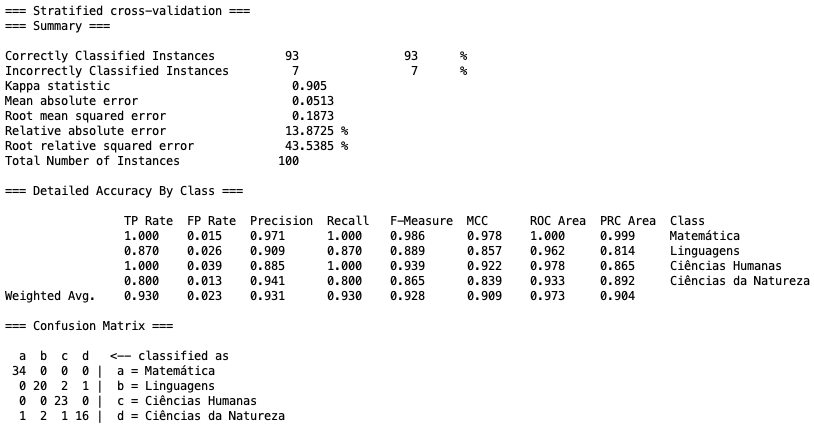
\includegraphics[width=16cm]{resources/resultado_treinamento.png} % leia abaixo
	\label{figura:rede}
	\captionsetup{singlelinecheck = false, format= hang, justification=raggedright, labelsep=space, width=16cm}
	\caption*{\footnotesize Fonte: O Autor.}
\end{figure}

A disposição da rede foi definida com três camadas escondidas, tal como mostra a figura \ref{figura:rede}.

\begin{figure}[H]
	\caption{Disposição da rede em camadas.}
	\centering % para centralizarmos a figura
	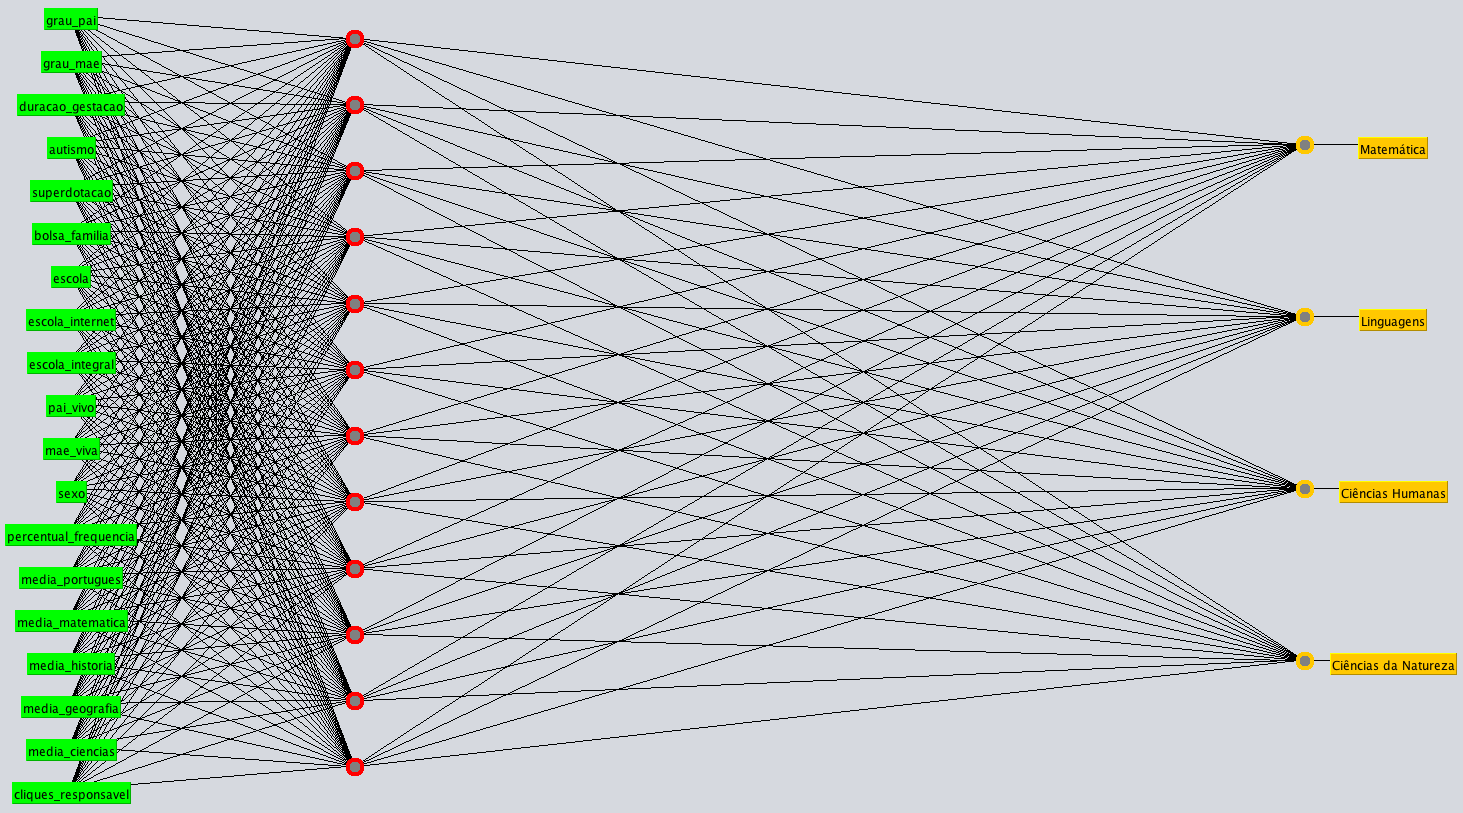
\includegraphics[width=16cm]{resources/rede.png} % leia abaixo
	\label{figura:rede}
	\captionsetup{singlelinecheck = false, format= hang, justification=raggedright, labelsep=space, width=16cm}
	\caption*{\footnotesize Fonte: O Autor.}
\end{figure}

\subsection{Implementar o módulo junto ao web service do aplicativo}

O processo de treinamento da rede foi realizado utilizando 

\section{Avaliação do Software}

Foi realizado avaliação do software construído através de pesquisa realizada com alunos do ensino médio integrado do Ifes Campus Cachoeiro de Itapemirim. 

\begin{figure}[H]
	\caption{Avaliação do aplicativo por alunos do ensino médio do IFES Campus Cachoeiro.}
	\centering % para centralizarmos a figura
	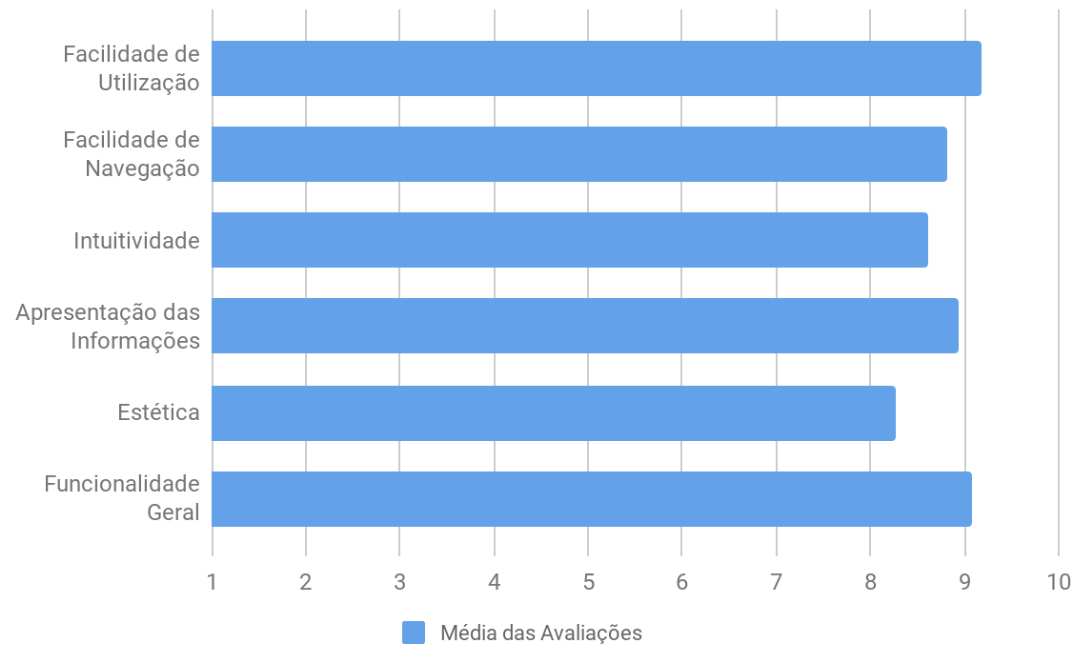
\includegraphics[width=15cm]{resources/pesquisa_avaliacao.png} % leia abaixo
	\label{figura:avaliacao}
	\captionsetup{singlelinecheck = false, format= hang, justification=raggedright, labelsep=space, width=15cm}
	\caption*{\footnotesize Fonte: O Autor.}
\end{figure}